\documentclass[11pt]{report}
\usepackage[english]{babel}
\usepackage[utf8x]{inputenc}

\newcommand{\me}{\mathrm{e}}
\usepackage{amsmath}
\usepackage{tabularx}
\usepackage{setspace}
\usepackage{natbib}
\usepackage{multicol}
\usepackage{amssymb}
\usepackage{ragged2e}
\usepackage{graphicx}
\usepackage[toc,page]{appendix}
\usepackage[colorinlistoftodos]{todonotes}
\usepackage[nottoc]{tocbibind}

\oddsidemargin 1.48cm
\evensidemargin .5cm

\begin{document}

\begin{titlepage}
\author{Sidharth S}
\newcommand{\HRule}{\rule{\linewidth}{0.5mm}}

\center % Center everything on the page
 
% Name of your university/college
\textsc{\LARGE \textbf{ImageNet Classification with\\[0.25cm] Deep Convolutional Neural Networks\\[0.99cm]}} % Major heading 

{ \it A seminar report submitted to Rajagiri School of Engineering \& Technology\\ in partial fulfilment of degree of \\[0.75cm]B.Tech.\\[0.5cm]}{in\\[0.5cm] Electronics \& Communication Engineering\\[0.75cm]by}\\[0.5cm]\textsc{\textbf{Sidharth S \\[0.35cm]Roll No: RET17EC146}}\\[1cm] % Minor heading such as course title



\includegraphics[width=2.5cm]{Rset Vertical.jpg}\\[1cm]
 
\textsc{DEPARTMENT OF ELECTRONICS \& COMMUNICATION ENGINEERING\\[0.15cm]\textsc{\textbf{RAJAGIRI SCHOOL OF ENGINEERING \& TECHNOLOGY}}\\[0.15cm]kerala\\[0.15cm]}{JANUARY 2021}
\thispagestyle{empty}
\end{titlepage}

\vfill % Fill the rest of the page with whitespace
\thispagestyle{empty}

\vspace*{-0.3cm}
\begin{center}
{\large \bf  DEPARTMENT OF ELECTRONICS \& COMMUNICATION ENGINEERING}\vspace{0.1cm}
\end{center}

\begin{center} 
{\Large \bf RAJAGIRI SCHOOL OF ENGINEERING \& TECHNOLOGY}\vspace{0.1cm}
\end{center}

\begin{center} 
{\large \bf KOCHI - 682039, }\vspace{0.1cm}
\end{center}

\begin{figure}[hbt]
\centering
\centerline{
\includegraphics[scale=0.6]{Rset Vertical.jpg}}
\end{figure}

\begin{center} 
{\Large \textit {Certificate}}\vspace{.1cm}
\end{center}

\justify
\doublespace
\textit {This is to certify that this report entitled ``ImageNet Classification with Deep Convolutional Neural Network'' is a bonafide record of the seminar presented by \textbf{Mr. Sidharth S, Roll No. RET17EC146} under our guidance towards the partial fulfilment of the requirements for the award of \textbf{Bachelor of Technology in Electronics \& Communication Engineering} of the \textbf{APJ Abdul Kalam Technological University}.}
\\[1cm]

\begin{minipage}{0.45\textwidth}
\begin{flushleft} \large
\textbf{Mr. Abhishek Viswakumar}\\
Assistant Professor\\
Dept. of ECE\\
RSET\\
Kochi
\end{flushleft}
\end{minipage}
~
\begin{minipage}{0.4\textwidth}
\begin{flushright} \large
\textbf{Dr. Rithu James}\\
HOD\\
Dept. of ECE\\
RSET\\
Kochi
\end{flushright}
\end{minipage}\\
~

\pagenumbering{roman}
\chapter*{Acknowledgement}
\setcounter{page}{1}
\addcontentsline{toc}{chapter}{Acknowledgement}
I am extremely grateful to \textbf{Prof.(Dr.) Sreejith P S}, Principal, Rajagiri School of Engineering and Technology, and \textbf{Dr. Rithu James}, Head of the Department, Electronics and Communication Engineering, for providing all the required resources for the successful completion of my seminar. My heartfelt gratitude to my seminar guide \textbf{Mr. Abhishek Viswakumar, Asst. professor, RSET} and seminar coordinators, \textbf{Mr. Naveen N, Ms. Mariya Vincent and Dr. Simi Zerine Sleeba} for their valuable suggestions and guidance. I express my sincere thanks to all staff members and friends for their help and co-ordination in bringing out this seminar successfully in time. I also acknowledge thankfully, the authors of the references and other literatures referred to in this seminar. Thank you.



\chapter*{Abstract}
\addcontentsline{toc}{chapter}{Abstract}
\doublespacing
Deep Convolutional Neural Networks\textit{(CNNs)} are used widely in the area of computer vision and image processing today and thus it is becoming increasingly important to have a comprehensive understanding of how they work. AlexNet introduced in the year 2012 has been ground breaking in the world of computer vision. This network is capable of classifying images into any one of the pre defined 1000 classes. The network consists of about 60 million parameters and 650,000 neurons. The various layers such as Convolutional Layers, Maxpooling layers, Fully connected layers and Softmax layers have been used in the network and these are all a part of the subjects for study in this seminar. The importance of activation functions and in particular, the ReLU activation function is also discussed along with other important topics such as dropout regularization which is used in the network. Study of AlexNet gives a comprehensive insight into the world of convolutional neural netwroks thus cementing the basics for diving into the world of computer vision.

\newpage
%\phantomsection
%\addcontentsline{toc}{chapter}{Acknowledgement}
%\phantomsection
%\addcontentsline{toc}{chapter}{Abstract}
\tableofcontents
\listoffigures
%\begingroup
%\let\clearpage\relax
\listoftables
%\endgroup
%\thispagestyle{empty}
%\listoffigures
%\listoftables

\newpage
\pagenumbering{arabic}
\chapter{Introduction}
Deep neural nets are widely in use today for a variety of machine learning purposes. Deep CNNs are usually used in the field of computer vision for applications such as object detection, face recognition, neural style transfer etc. The seminar deals with the study of AlexNet, a pioneer in the field of deep convolutional neural networks. This will provide us a intuition as to why CNNs are useful for image processing applications.
\section{Introduction to AlexNet}
The model under study is termed 'AlexNet' after the creator of the network, Alex Krizhevsky. He was working at the University of Toronto along with the co-authors Ilya Sutskever and Geoffrey E. Hinton.

AlexNet is considered one of the most influential papers published in computer vision, having spurred many more papers published employing CNNs and GPUs to accelerate deep learning. As of 2020, the AlexNet paper has been cited over 70,000 times according to Google Scholar. \citep{one}

 Convolutional Neural Networks (CNNs) had always been the go-to model for object recognition — they’re strong models that are easy to control and even easier to train. They don’t experience overfitting at any alarming scales when being used on millions of images. Their performance is almost identical to standard feedforward neural networks of the same size. AlexNet is the first Convolutional Neural Network (CNN) where multiple convolution
operations were used.
 
\section{Dataset: ImageNet}
 ImageNet is a dataset made of more than 15 million high-resolution images labeled with 22 thousand classes. The key: web-scraping images and crowd-sourcing human labelers. ImageNet even has its own competition: the ImageNet Large-Scale Visual Recognition Challenge (ILSVRC). This competition uses a subset of ImageNet’s images and challenges researchers to achieve the lowest top-1 and top-5 error rates (top-5 error rate would be the percent of images where the correct label is not one of the model’s five most likely labels). In this competition, data is not a problem; there are about 1.2 million training images, 50 thousand validation images, and 150 thousand testing images.
 
\subsection{The ImageNet Large Scale Visual Recognition Challenge (ILSVRC)} \label{ilsvrc}
The ImageNet Large Scale Visual Recognition Challenge (ILSVRC) evaluates algorithms for object detection and image classification at large scale. One high level motivation is to allow researchers to compare progress in detection across a wider variety of objects -- taking advantage of the quite expensive labeling effort. Another motivation is to measure the progress of computer vision for large scale image indexing for retrieval and annotation.

AlexNet was originally developed by the authors to take part in the ILSVRC challenge. The performance of the network is also benchmarked with this competition and compared with the other competitors. The authors of the paper has discussed in detail about this in the original paper. \citep{one}

\chapter{A Comprehensive Study of Convolutional Neural Networks}
Before going into more details about AlexNet, it is imperative to know a few basic details about CNNs. This secction serves the purpose of providing the necessary insight into the working of CNNs so as to help the study AlexNet in detail.

\section{Need for CNNs in Computer Vision}
Fully connected neural networks (\textit{FCNNs}) are a type of neural network where the
architecture is such that all the nodes, or neurons, in one layer are connected to the neurons in the next layer. Fully connected neural networks are used for a wide variety of applications in the world of deep learning. But studies have shown that FCNNs cannot be used in computer vision applications due to a number of reasons. FCNNs involve a lot of computations, especially for datasets involving images. \textit{For eg:} A simple 128 x 128 x 3 image given as a input would require \textit{151, 875} units just at the first layer of the network.

There exists other problems such as overfitting, slower time for gradient descent in networks having a large number of parameters. So it can be concluded that FCNNs are not the ideal solution in the case of computer vision applications and thus arises the need for CNNs.

\section{Convolutional Neural Networks}
\subsection{Convolution Operation}
In mathematics, convolution is a mathematical operation on two functions $f$ and $g$ that
produces a third function $f \ast g$ that expresses how the shape of one is modified by the other as seen in equation \ref{convop}. 

Mathematically,
\begin{equation} \label{convop}
(f \ast g)(t) \triangleq \int_{-\infty}^{\infty} f(\tau)g(t-\tau)d\tau
\end{equation}


\subsection{Convolution Operation in CNNs}
In the case of a CNN, the convolution is performed on the input data, which is an image, with the use of a \textbf{filter} or \textbf{kernel} (these terms are used interchangeably) to then produce a feature map.
\begin{figure}[!h] 
	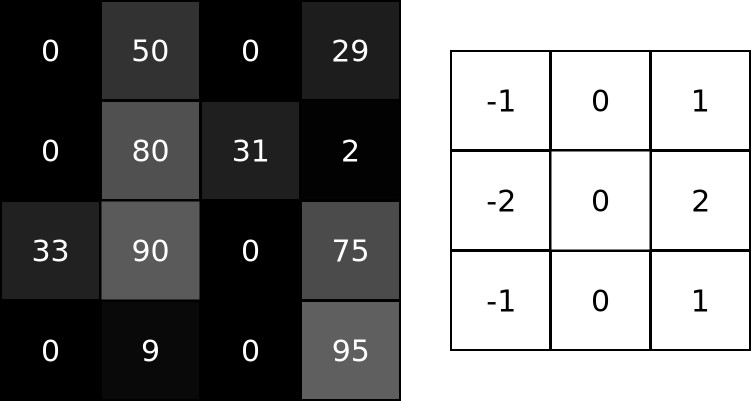
\includegraphics[scale=0.3]{convexample1.png} 
	\centering 
	\caption{An Example - A 4x4 image (left) and a 3x3 Sobel filter (right)}
	\label{convex}
	%\vspace{3pt}
\end{figure}
An input image and a filter can be used to produce an output image by convolving the
filter with the input image. The steps for convolutions are:
\begin{enumerate}
	\item Overlaying the filter on top of the image at some location.
	\item Performing \textbf{element-wise multiplication} between the values in the filter and their corresponding values in the image.
	\item Summing up all the element-wise products. This sum is the output value for the destination pixel in the output image.
	\item Repeating for all locations.
\end{enumerate}

Figure \ref{convex} shows an example of a convolution operation. Figure \ref{outputpic} shows the corresponding output.
\begin{figure}[!h]
	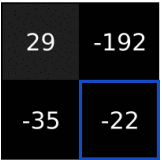
\includegraphics[scale=0.5]{convop.png}
	\centering
	\caption{Output of the convolution operation}
	\label{outputpic}
	%\vspace{3pt}
\end{figure}
Using a filter smaller than the input is intentional as it allows the same filter (set of weights) to be multiplied by the input array multiple times at different points on the input. Specifically, the filter is applied systematically to each overlapping part or filter-sized patch of the input data, left to right, top to bottom.

\subsection{Kernals or Filters}
The systematic application of the same filter across an image is a powerful idea. If the filter is designed to detect a specific type of feature in the input, then the application of that filter systematically across the entire input image allows the filter an opportunity to discover that feature anywhere in the image. This capability is commonly referred to as \textbf{translation invariance.}

In figure \ref{convex}, we saw an example of convolution with the \textit{Sobel filter}. Sobel filter is an example of an edge detector. It can be used to detect either horizontal or vertical edges present in an image. It works by calculating the gradient of image intensity at each pixel
within the image. It finds the direction of the largest increase from
light to dark and the rate of change in that direction.
The result shows how abruptly or smoothly the image changes at each
pixel, and therefore how likely it is that that pixel represents an edge. Figure \ref{kernalex} shows the result after applying Sobel filter to an image.

\begin{figure}[!h]
	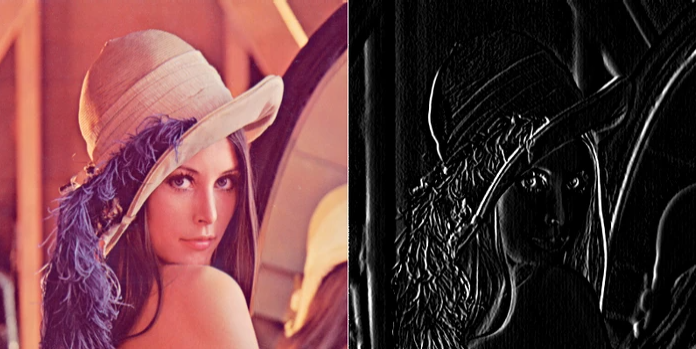
\includegraphics[scale=0.4]{filter.png}
	\centering 
	\caption{An image convolved with the vertical Sobel filter.}
	\label{kernalex}
\end{figure}
\vspace{7pt}
Thus kernels can detect features on a global scale anywhere in the image. While Sobel filters are used to find edges, filters to find other required features, say, occurrence of a particular object in the image (object detection) can be learned using machine learning. For this, we can give random weight matrices instead of fixed values for the filters and we can make the network learn from a certain dataset.

\subsection{Padding and Stride}
\subsubsection{Padding}
One issue when applying convolutional neural networks is that we tend to lose pixels on the perimeter of our image.

Assuming that the input shape is $k_h \times k_w$, then the output shape will be $(n_h - k_h + 1)\times(n_w - k_w +1)$.
It can be observed that the output of the convolutional layer is shrunk. Especially in deep CNNs, the successive convolution operations may lead to the output layer being very small and hence affecting the learning of the network.  One straightforward solution to this problem is to add extra pixels of filler around the boundary of our input image, thus increasing the effective size of the image. Typically, we set the values of the extra pixels to zero. Figure \ref{paddingex} shows how padding is applied to the example in figure \ref{convex}.

\begin{figure}[!h]
	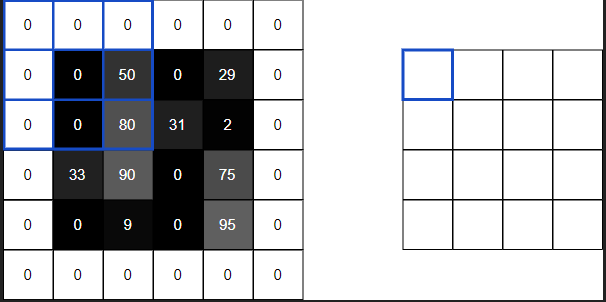
\includegraphics[scale=0.5]{padding.png}
	\centering 
	\caption{Example of padding.}
	%\vspace{3pt}
	\label{paddingex}
\end{figure}
In general, adding a total of  $p_h$ rows of padding (roughly half on top and half on bottom) and a total of  $p_w$  columns of padding (roughly half on the left and half on the right), the output shape will be given by equation \ref{paddingeq}
\begin{equation} \label{paddingeq}
(n_h - k_h + p_h + 1) \times (n_w - k_w + p_w + 1)
\end{equation}

\subsubsection{Stride}
When computing the convolution, we start with the convolution window at the top-left corner of the input tensor, and then slide it over all locations both down and to the right. In previous examples, we default to sliding one element at a time. However, sometimes, either for computational efficiency or because we wish to down sample, we move our window more than one element at a time, skipping the intermediate locations.

We refer to the number of rows and columns traversed per slide as the \textit{stride}. In general, when the stride for the height is $s_h$ and the stride for the width is $s_w$ , the output shape is given by equation \ref{strideeq}
\begin{equation} \label{strideeq}
\lfloor (n_h - k_h + p_h + s_h)\ /\ s_h\rfloor \times \lfloor (n_w - k_w + p_w + s_w)\ /\ s_w \rfloor
\end{equation}


\section{Maxpool layers} \label{maxpool}
A problem with the output feature maps is that they are sensitive to the location of the features in the input. One approach to address this sensitivity is to down sample the feature maps. This has the effect of making the resulting down sampled feature maps more robust to changes in the position of the feature in the image, referred to by the technical phrase \textit{“local translation invariance.”}

Pooling layers provide an approach to down sampling feature maps by summarizing the presence of features in patches of the feature map. Two common pooling methods are average pooling and max pooling that summarize the average presence of a feature and the most activated presence of a feature respectively. Maxpool layers does not have any parameters to learn.

\begin{figure}[!h]
	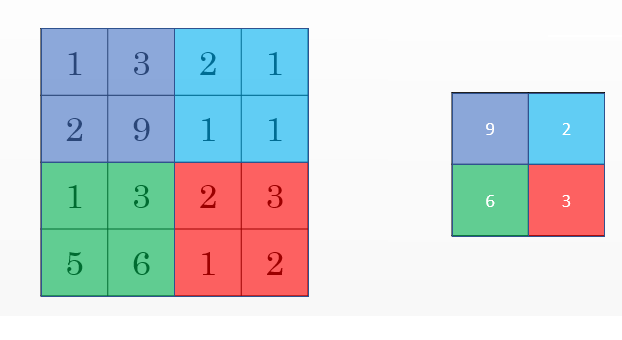
\includegraphics[scale=0.32]{maxpool.png}
	\centering 
	\caption{Example of a maxpool layer}
	\label{maxpoolex}
	%\vspace{3pt}
\end{figure}

The maxpool layer is basically saying, if the feature is detected anywhere in this filter then keep a high number. This can be observed in figure \ref{maxpoolex}. Thus the objective of the maxpool layer is to take care of the redundant information as the neighboring pixels in images tend to have similar values. It also helps in reducing the spatial dimension of the input volume for next layers. AlexNet makes use of maxpool layers.

\section{Activation Functions}
The activation function is the non-linear transformation that we do over the input signal. This transformed output is then sent to the next layer of neurons as input. Activation function enables the network to learn complex patterns in the dataset given to it.
\subsubsection{Need for activation function}
Activations are an essential part in neural networks for a number of reasons. The primary reason as discussed earlier is that without activation functions, the network can learn only linear relationship between data. So no matter how deep the network is, it still amounts to a linear regression model as all layers will behave same way because the composition of two linear function is a linear function itself. As most of the features we need the network to train on amounts to non-linear distribution, non linear activations functions are indispensable. 

Activation functions also help in keeping the value of the output from the neuron restricted to a certain limit as per our requirement. This is important because input into the activation function is $W*x + b$ where $W$ is the weights of the cell and the $x$ is the inputs and then there is the bias $b$ added to that. This value if not restricted to a certain limit can go very high in magnitude especially in case of very deep neural networks that have millions of parameters. This will lead to computational issues.

\chapter{AlexNet}
\section{Architecture}
\begin{figure}[!h]
	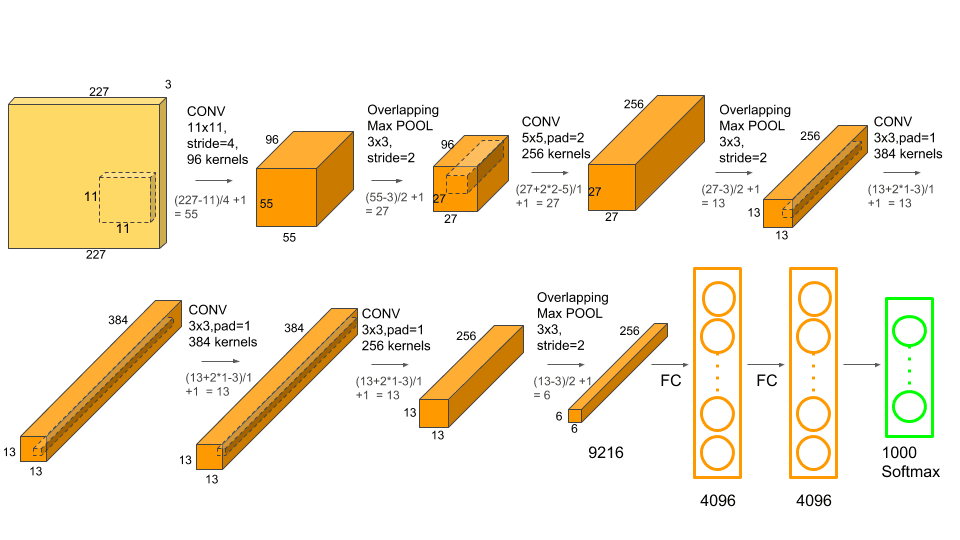
\includegraphics[scale=0.32]{architecture.png}
	\centering 
	\caption{Architecture of AlexNet}
	\label{archi}
	%\vspace{3pt}
\end{figure}

Now we are ready to describe the overall architecture of our CNN. As depicted in Figure \ref{archi}, the net contains eight layers with weights; the first five are convolutional and the remaining three are fullyconnected. The output of the last fully-connected layer is fed to a 1000-way softmax which produces a distribution over the 1000 class labels. The neurons in the fullyconnected layers are connected to all neurons in the previous layer. Max-pooling layers of the kind described in section \ref{maxpool} is also used.

The first convolutional layer filters the 227×227×3 input image with 96 kernels of size 11×11×3 with a stride of 4 pixels. The second convolutional layer takes as input the  output of the first convolutional layer and filters it with 256 kernels of size 5×5×48.
The third, fourth, and fifth convolutional layers are connected to one another without any intervening
pooling or normalization layers. The third convolutional layer has 384 kernels of size 3×3×256 connected to the outputs of the second convolutional layer. The fourth
convolutional layer has 384 kernels of size 3×3×192 , and the fifth convolutional layer has 256
kernels of size 3×3×192. The fully-connected layers have 4096 neurons each.

In the following sections, the architecture and different features of the network are discussed in detail.

\section{Dataset}
ImageNet is a dataset of over 15 million labeled high-resolution images belonging to roughly 22,000 categories. The images were collected from the web and labeled by human labelers using Amazon’s Mechanical Turk crowd-sourcing tool.  ILSVRC (see section \ref{ilsvrc}) uses a subset of ImageNet with roughly 1000 images in each of 1000 categories. In all, there are roughly 1.2 million training images, 50,000 validation images, and 150,000 testing images.

\section{ReLU Nonlinearity}
ReLU nonlinearity is an activation function which is widely in use today. AlexNet was one of the factors which popularised the use of ReLU nonlinearity in neural networks. The popularity of ReLU activation function can be attributed to some factors which are discussed in this section.

\begin{equation} \label{relueq}
	f(x) =
  				\begin{cases}
    			0       & \quad \text{for } x\ <\ 0\\
    			x  & \quad \text{for } x\ \geq\ 0
  				\end{cases}
\end{equation} 
  				

The rectified linear activation function or ReLU for short is a piecewise linear function that will output the input directly if it is positive, otherwise, it will output zero. This can be observed from equation \ref{relueq}.  
				It has become the default activation function for many types of neural networks because a model that uses it is easier to train and often achieves better performance.
\begin{figure}[!h]
	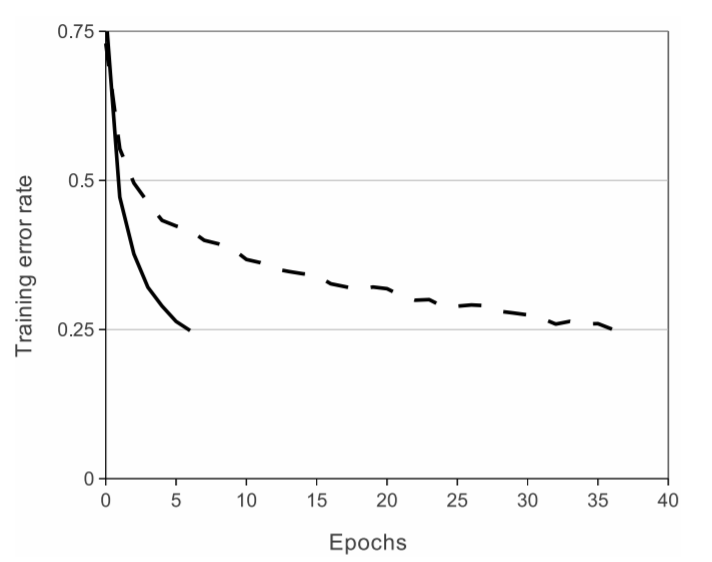
\includegraphics[scale=0.4]{relu.png}
	\centering 
	\caption{Error of a four layer convolutional neural network with ReLU activation.}
	\label{relu}
\end{figure}

Deep convolutional neural networks with ReLUs train several times faster than their equivalents with tanh units. This is demonstrated in Figure \ref{relu}, which shows the number of iterations required to reach 25\% training error on the CIFAR-10 dataset for a particular four-layer convolutional network. The network trained with ReLU (solid line) attains error rate much faster than a network using sigmoid activation (dashed line). This plot shows that a neural network as large as AlexNet would not be possible with traditional activation functions such as tanh.

\section{Reducing Overfitting}
Since the network is large with over 60 million parameters, even the 1000 classes of the image data set was found to be insufficient to learn so many parameters without considerable overfitting. Overfitting is demonstrated in figure \ref{overfit}. Two methods are in use in AlexNet to combat overfitting.

\begin{figure}[!h]
	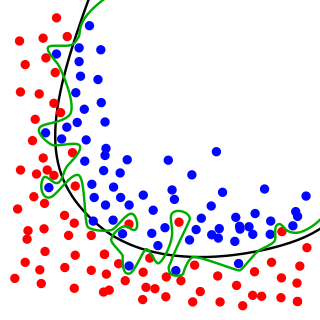
\includegraphics[scale=0.3]{overfit.png}
	\centering 
	\caption{Example of overfitting - Black line fits the data well. Green is overfitting.}
	\label{overfit}
	%\vspace{3pt}
\end{figure}

\subsection{Data Augmentation}
The easiest and most common method to reduce overfitting on image data is to artificially enlarge the dataset using label-preserving transformations. Data augmentation is a technique to increase the diversity of your training set by applying random (but realistic) transformations such as image rotation. AlexNet employ two distinct forms of data augmentation, both of which allow transformed images to be produced from the original images with very little computation, so the transformed images do not need to be stored on disk. In our implementation, the transformed images are generated in Python code on the CPU while the GPU is training on the previous batch of images. So these data augmentation schemes are, in effect, computationally free.

\subsection{Dropout Regularization}
Dropout is a regularization method that approximates training a large number of neural networks with different architectures in parallel.

During training, some number of layer outputs are randomly ignored or “dropped out.” This has the effect of making the layer look-like and be treated-like a layer with a different number of nodes and connectivity to the prior layer. In effect, each update to a layer during training is performed with a different “view” of the configured layer.

This technique reduces complex co-adaptations of neurons,
since a neuron cannot rely on the presence of particular other neurons. It is, therefore, forced to
learn more robust features that are useful in conjunction with many different random subsets of the
other neurons. At test time, the network use all the neurons but multiply their outputs by 0.5, which is a reasonable approximation to taking the geometric mean of the predictive distributions produced by the exponentially-many dropout networks. 

AlexNet use dropout in the first two fully-connected layers of Figure \ref{archi}. Without dropout, our network exhibits substantial overfitting. Dropout roughly doubles the number of iterations required to converge.

\chapter{Results and Observations}
The study of AlexNet gives an insight into the complex world of deep neural networks.

From table \ref{tab}, it can be observed how the AlexNet performs on the ILSVRC - 2010 dataset. The study of performance of AlexNet was done from the results given in the paper \citep{one}.
%\vspace{15pt}
		\begin{table}[!h]
		\begin{tabular}{||c| c| c||} 
	 	\hline
 		\textbf{Model} & \textbf{Top-1} & \textbf{Top-5} \\ [0.5ex] 
 		\hline\hline
 		\textit{Sparse Coding} & \textit{47.1\%} & \textit{28.2\%}\\ 
 		\hline
 		\textit{SIFT + FVs [24]} & \textit{45.7\%} & \textit{25.7\%} \\
 		\hline
 		CNN & \textbf{37.5\%} & \textbf{17.0\%}\\
 		\hline
 	\end{tabular}
 	\centering
 	\caption{Comparison of results on ILSVRC-2010 test set. In italics are best results
achieved by others.}
\label{tab}
	\end{table}

\newpage

\begin{figure}[!h]
	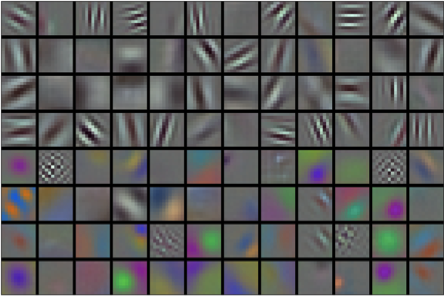
\includegraphics[scale=0.3]{learning.png}
	\centering 
	\caption{96 convolutional kernels of size
11×11×3 learned by the first convolutional
layer on the 224×224×3 input images.}
	\label{learn}
\end{figure}

Figure \ref{learn} shows the convolutional kernels learned by the networks two data-connected layers. The
network has learned a variety of frequency- and orientation-selective kernels, as well as various coloured blobs. The learning process of the network was also observed and studied accordingly.


\begin{figure}[!h]
	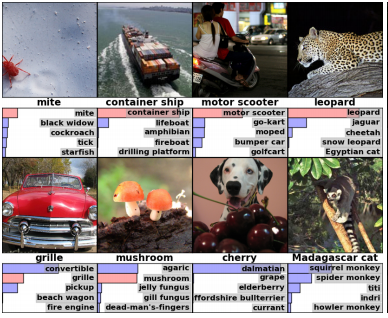
\includegraphics[scale=0.85]{result.png}
	\centering 
	\caption{Eight ILSVRC-2010 test images and the five labels considered most probable by the model.}
	\label{result}
\end{figure}

The model was found to have very good performance on the dataset provided.\citep{one} Figure \ref{result} shows us how AlexNet classifies images from the ImageNet dataset. The correct label is written under each image, and the probability assigned to the correct label is also shown with a red bar (if it happens to be in the top 5). It can be observed how the network predicts labels for the images and classifies them.

 Use of ReLU activation and multiple GPUs enabled the network to train faster. Regularisation with dropout was found to be essential to prevent overfitting.
%\chapter{Observations}
%
%\begin{figure}[!h]
%	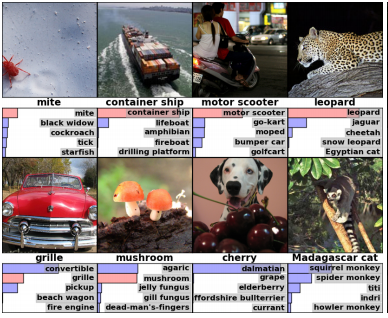
\includegraphics[scale=0.85]{result.png}
%	\centering 
%	\caption{Eight ILSVRC-2010 test images and the five labels considered most probable by the model.
%The correct label is written under each image, and the probability assigned to the correct label is
%also shown with a red bar (if it happens to be in the top 5).}
%	\label{result}
%\end{figure}
%
%The model was found to have very good performance on the dataset provided. Use of ReLU activation and multiple GPUs enabled the network to train faster. Regularisation with dropout was found to be essential to prevent overfitting.

\chapter{Conclusion}
AlexNet was a pioneer in the field of computer vision and opened up a whole new research era. Dropout, ReLU, and deep layers are key steps in achieving excellent performance in computer vision task and removing any of the convolutional layers will drastically degrade the performance of the network. This indicated that deep learning is useful for machine learning tasks for computer vision as well as other applications.

Further studies regarding deep convolutional networks were done following the inception of AlexNet. This includes GoogleNet, which was the winner of ILSVRC 2014 developed by engineers at Google. ResNet, the winner of ILSVRC 2015 with a top-5 error rate of just 3.5\% which beat human level performance on the dataset was the result of the research whose foundations were based on AlexNet.

Thus even today, AlexNet still remains relevant as it is the basis for many of the new developments in the field of computer vision. 

\bibliographystyle{unsrt}
\bibliography{references.bib}
\cite{one}
\cite{two}
\cite{three}
\cite{four}
\cite{five}
%\section{Baseline Vehicle -Toyota Prius}
%In this study ,Toyota Prius 2004 model is taken as the baseline vehicle.The torque speed envelope is as shown in.Here ,peak torque is 300Nm up to base speed of 1500 rpm and high torque of 60Nm at maximum speed o 6000rpm.Maximum dc-link voltage is 500V.
%\begin{center}
%
%\begin{figure}[!hbt]
%\centering
%\includegraphics[width=6cm]{bb.pdf}
%
%\caption{baseline torque speed characteristics}
%\end{figure}
%
%\end{center}
%
%\section{Motor Topologies}
%Four different motor topologies are selected for comparison : interior permanent magnet synchronous motor with 48-slot 8-pole (48/8 IPMSM) ,IPMSM with 12 slot 8-pole (12/8 IPMSM) ,induction motor with 48-slot 36 rotor bar (48/36 IM) and switched reluctance motor with 12-slot 8-pole (12/8 SRM).
%
%
%
%
%\begin{table}[!hbt]
%\centering
%
%\label{table 1}
%\begin{tabular}{|p {2cm}| r| r| r| r| }
%\hline
%parameter &48/8IPMSM &12/8 IPMSM&48/36 IM&12/8 SRM \\\hline
%Max. dc-link voltage(V)&500&500&500&500\\\hline
%Max. rotational speed (rpm)&6000&6000&6000&6000\\\hline
%peak power (kW)&50&50&50&50\\\hline
%
%designed Torque(Nm) &100&120&90&100\\\hline
%operating point speed(rpm)&3000&2500&3300&3000\\\hline
%pole pairs&4&4&2&-\\\hline
%stator outer diameter(mm) &269&269&269&269\\\hline
%Stator inner diameter (mm) &161.9&166&177.9&172\\\hline
%Rotor inner diameter(mm) &110&100&94&90\\\hline
%
%
%\end{tabular}
%\caption{motor topologies}
%\end{table}
%
%
%
%
%\section{Analysis of motor topologies}
%\subsection { IPMSM}
%Transient 2-D analysis is used for both configurations of IPMSM.the method is as explained for 48/8 IPMSM:\\ Injecting currents into the winding, motor parameters need to be extracted, especially the flux linkage. Fig.~\ref{d-axis} and Fig.~\ref{q-axis} show Prius motor’s d-axis and q-axis flux linkage at different current levels respectively. \\ Based on the flux linkage information, optimal operating plane needs to be generated, as shown in Fig.~\ref{48}. This plane is bounded by current limit circle, maximum torque per ampere (MTPA) curve and maximum torque per voltage (MTPV) curve. Constant torque loci (black curves) and voltage ellipse (blue dotted curves) have also been shown. \\ For each given torque speed requirement, optimal current$ i_d $and $i_q $can be determined by using extrapolation and interpolation techniques. 
%The same steps are repeated for 12/8 IPMSM. 
%
%\begin{figure}[!hbt]
%\includegraphics[width=6cm]{cc.pdf}
%\caption{d-axis flux linkage at different current levels for 48/8 IPMSM}
%\label{d-axis}
%\end{figure}
%\begin{figure}[!hbt]
%\includegraphics[width=6cm]{dd.pdf}
%\caption{q-axis flux linkage at different current levels for 12/8 IPMSM}
%\label{q-axis}
%\end{figure}
%\begin{figure}[!hbt]
%\includegraphics[width=6cm]{48-8_ipmsm.pdf}
%\caption{optimal operating plane for 48/8 IPMSM}
%\label{48}
%\end{figure}
%\begin{figure}[!hbt]
%\includegraphics[width=6cm]{ff.pdf}
%\caption{optimal operating plane for 12/8 IPMSM}
%\label{12}
%\end{figure}
%\newpage
%
%\subsection{48/36 IM}
%Compared to the 48/8 IPMSM, 48/36 IM has longer stack length (108mm) to achieve large torque and high efficiency design. FEA transient analysis of induction machine requires significant computation time, especially when the excitation is provided by a voltage source. The current needs several periods to reach steady state. To reduce computation time, Instead of applying voltage in stator winding while keeping rotor copper bar short-circuited, both stator and rotor currents are injected into stator winding and rotor copper bar individually. In the rotor flux reference frame, when the Field Oriented Condition (FOC) is satisfied, which means only the d-axis rotor flux exists while q-axis rotor flux is zero.(Appendix 1)i.e.,\begin{equation} \label{1} \lambda_r=\lambda_{rd} \end{equation}
%where $\lambda_r$ is rotor flux ,$\lambda_{rd}$ is rotor direct axis flux,$\lambda_s$ is stator flux ,$I_s $ is stator current 
%\begin{figure}[!hbt]
%\includegraphics[width=9cm]{kk.pdf}
%\caption{d-axis flux linkage at different current levels}
%\label{foc}
%\end{figure}
%\\ The fast FEA modeling approach based on current excitation consists of  Magneto static FEA modeling where Both stator and rotor currents are injected into the stator winding and rotor copper bar separately. The q-axis currents are adjusted iteratively until FOC is satisfied as shown in Eq.~\ref{1}. Machine parameters including stator inductance$ L_s$, rotor inductance $L_r$, and mutual inductance$ L_m$ can be calculated based on current and flux information. \\
%\subsection{12/8 SRM}
%
% Transient 2-D analysis in Maxwell is used with circuit field coupling method for SRM.
% \begin{figure}[!hbt]
%\includegraphics[width=9cm]{gg.pdf}
%\caption{flux linkage and static torque profile at different rotor positions for SRM}
%\label{angle control}
%\end{figure}
%
%    The turn-on angle, turn-off angle and current amplitude can be used to optimize SRM efficiency over full torque-speed range .To keep it simple, the control strategy was designed as follows- At low speed, current chopping control was adopted with fixed turn-on angle and fixed dwell angle; at medium speed, current chopping control is adopted with fixed dwell angle and variable turn-on angle; at further high speed, angular position control (single pulse operation) with advancing turn on angle and fixed turn off angle is adopted.  
%
%\section{NVH Analysis}
% Modal Analysis of different motor topologies are done in ANSYS workbench environment. Radial Force due to  Electromagnetic radial force density acting on stator teeth causes deformation of stator yoke. Based on Maxwell stress tensor method, it is calculated as follows 
% 
%\begin{equation}
%f_{rad}(\theta,t)=\frac{B_r^2(\theta,t){-} B_t^2(\theta,t)}{2\mu_0}
%\end{equation}
%where $B_r$ and $B_t$ are radial and tangential components of air gap flux density,$\mu_0 $permeability of air ,$\theta$ angular position and $t$ time
% \begin{figure}[!hbt]
%\includegraphics[width=5cm]{vv.pdf}
%\caption{stator core deformation under different load conditions (a) 48/8 IPMSM (b)12/8 IPMSM (c)48/36 IM (d)12/8 SRM}
%\label{modal}
%\end{figure}
%\newpage
%\begin{table}[!hbt]
%\label{table 2}
%\centering
%\caption{Maximum deformation of the stator in$ \mu$ m}
%\begin{tabular}[p]{|l|l|l|l|l|l|}
%\hline Torque&speed&48/8 &12/8&48/36& 12/8\\ 
%Nm &rpm &IPMSM &IPMSM & IM &SRM\\\hline
%50&1000&0.584&5.17&0.727&5.19\\
%50&5000&0.495&3.80&0.645&4.72\\\hline
%\end{tabular}
%
%\end{table}
%Fig.~\ref{modal} shows the total deformation of stator core under different load conditions. Under the load 50Nm at 1000rpm, 48/8 IPMSM has the minimum stator core deformation with 5.84$\me^{-7}$m while 12/8 IPMSM and 12/8 SRM have the maximum deformation with 5.17$\me^{-6}$m. Under the load 50Nm at 5000rpm, 12/8 SRM has the maximum deformation with 4.72$\me^{-6}$m due to single pulse operation. For the other three motors, deformation is smaller than those under 50Nm at 1000rpm condition due to field weakening control at high speed. Table.2.2 compares the maximum deformation of stator under different load conditions. 
%
%\chapter{Results}
%\section {Noise vibration and harshness analysis} NVH show that 48/8 IPMSM offer quitest operation.While SRM is the noisiest as in table~\ref{table 2} .48/8 IPMSM has higher mode number (Appendix B) ,so less stator deformation as vibrational amplitude is inversely proportional to 
%fourth power of mode order.
%
%\section{Transient analysis}
%When operating planes for 48/8 IPMSM figure~\ref{48} and 12/8 IPMSM figure~\ref{12} are compared, it is seen that for 12/8 IPMSM maximum torque per ampere line shifts away into  $i_q${>}$i_d$ region.This means electromagnetic torque dominates.12/8 IPMSM has low saliency and reluctance torque is not fully utilized.
%\chapter{Observations}
%In induction machines with squirrel-cage  dominant losses are copper loss.The required magnetization current and copper losses in rotor decrease efficiency in the range of nominal speed compared to PMSM.A disadvantage is the heat in the rotor as a result of the losses, which requires cooling and restricts overload capacity. Furthermore, an air gap as small as possible is necessary to decrease the magnetization current, but this requires tighten tolerances during fabrication and thus increases production costs.\\
%The excitation of the PMSM is provided by permanent magnets in the rotor. This machine benefits from the high energy density of the magnets, because the permanent magnet excitation requires little space. Since no excitation current is required, the PMSM provides a high overall efficiency in the range of nominal speed. The dominant losses of the PMSM are the iron losses, which mostly occur in the stator, so they can be easily dissipated by a case cooling system. Hence, the PMSM exceeds the IM in power density and efficiency.\\
%The SRM provides a power density and efficiency comparable to the IM. However, it has a simple construction without rotor winding and with concentrated stator windings, and therefore a better thermal characteristic. In addition, it is cost-effective in production and low-maintenance. To reach a high power density, a high air-gap induction is recommended - this however increases acoustic noise radiation. Measures for noise reduction decrease the power density and diminish the appeal of the SRM compared to the IM Another disadvantage is the high torque ripple at low speeds.
%\chapter{Conclusions}
%To determine the most suitable electrical machine for hybrid electrical vehicles, several machine types were compared. It is concluded that  PMSM as the most suitable machine for parallel hybrid systems. A result which is confirmed by the fact, that the PMSM is the mostly used machine type of today's HEVs.Among the two configurations of IPMSM studied ,48/8 IPMSM was found to more efficient with least noise operation.Hence the use of IPMSM in Toyota Prius is justified.
%
%
%\newpage 
%
%\bibliographystyle{unsrt}
%\bibliography{references.bib}
%\cite{one}
%\cite{two}
%\cite{three}
%\cite{four}
%\cite{five}


\end{document}